\section{Introduction}	
% Explanation of title and why someone should read
This paper discusses an algorithm which can be used for indoor painting detection and localization. The input of this algorithm is a picture, preferably containing one or multiple paintings, and the output is the room of the museum where the picture was taken. The algorithm contains three contributions.

The first contribution is a method for extracting paintings from a picture using a combination of the Canny edge detector \cite{Canny1986} and Suzuki's method \cite{SUZUKI198532} for finding contours in an image. This combination allows to approximate a first polygon which encloses the painting. This polygon can be approximated into a similar polygon with fewer points using the Ramer–Douglas–Peucker algorithm \cite{Hershberger92speedingup}. Only polygons containing four point are considered, as they can represent the rectangular shape of the painting. This last polygon is used to transform the painting into a rectangle of predefined size.

The second contribution is a simple matching algorithm to compare the extracted painting against paintings in a database. It is inspired by the works of Rublee et al. \cite{Rublee2011} which uses Brute Force matching based on ORB. 

The final contribution of this paper is the usage of meta-data associated with the matched painting from the database. In our implementation, the meta-data is used to provide a strict way of localizing the painting and, by extension the user on a floor plan, as seen on figure \ref{fig:groundplan_msk}. The algorithm is not limited by this meta-data in its current state, as it can be expanded should the need arise.

% Results
The database of 688 paintings is matched every 30 frames with the videos running at 30 frames per second. All paintings are compressed to 1000 x 1000 pixels in order to speed up the matching procedure. In order to test the efficiency of our algorithm, a ground truth was established by taking a small sample of 30 paintings and manually labeling them. We achieved a segmentation accuracy of 47.10\% and a painting matching accuracy and subsequently localization accuracy of 46.67\%.

% Usefulness
If improved further, this algorithm could have multiple practical uses such as finding a fastest way out of the museum based on a screenshot, providing additional information about detected paintings, or finding other people inside the museum. 
%The algorithm's usefulness is not only limited to museums, any indoor location which contain many items of the same type, such as a guitar store or . 

\subsection{Overview}
The succeeding sections of this paper will discuss the implementation of the proposed algorithm. Section \ref{sec:painting_detection} will discuss the inner workings of the algorithm. Section \ref{sec:results} will describe the used performance metrics to evaluate the effectiveness of the algorithm, the experimental results and finish it up by presenting a qualitative analysis where the strengths and weaknesses of our proposed algorithm are laid bare. Section \ref{sec:conclusion} repeats the major contributions and results of this paper.


\begin{figure}
	\includegraphics[width=\linewidth, height=100pt]{flowchart}
	\caption{A flowchart of the algorithm.}
	\label{fig:flowchart}
\end{figure}
\begin{figure}
	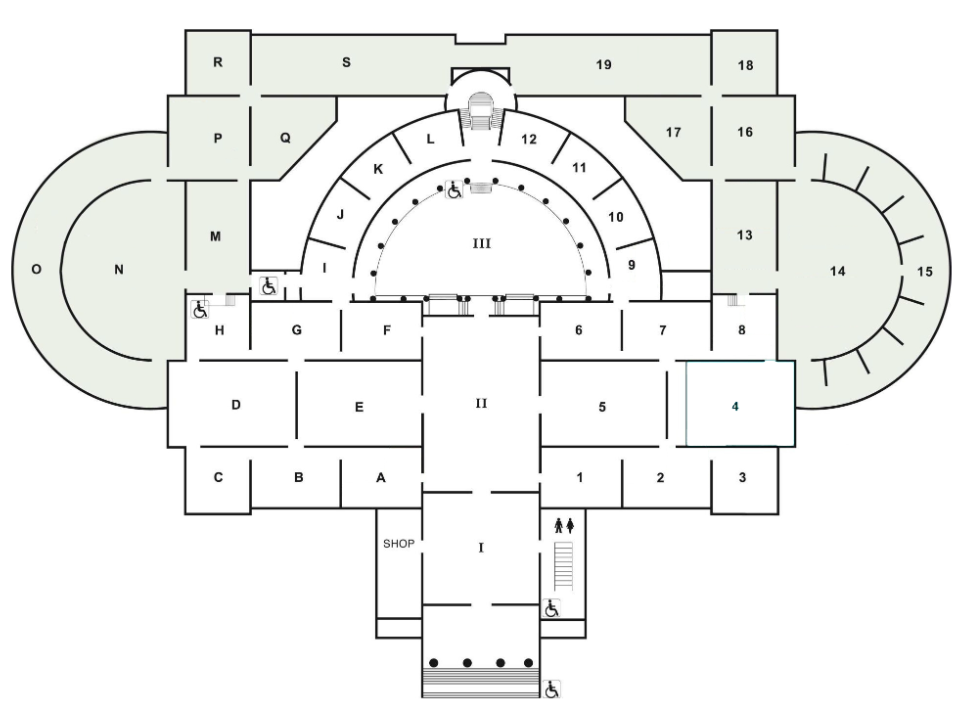
\includegraphics[width=\linewidth]{groundplan_msk}
	\caption{A ground plan of The Museum of Fine Arts, Ghent. }
	\label{fig:groundplan_msk}
\end{figure}